\documentclass{beamer}
\usepackage{tikz}
\usepackage{tikz-qtree}
\usepackage{gillius}
\usepackage{mathdots}
\usepackage{abraces}
\usepackage{etex}
\usepackage{array}
\usepackage[backend=biber]{biblatex}

% http://tex.stackexchange.com/questions/12703/how-to-create-fixed-width-table-columns-with-text-raggedright-centered-raggedlef
\newcolumntype{L}[1]{>{\raggedright\let\newline\\\arraybackslash\hspace{0pt}}m{#1}}
\newcolumntype{C}[1]{>{\centering\let\newline\\\arraybackslash\hspace{0pt}}m{#1}}
\newcolumntype{R}[1]{>{\raggedleft\let\newline\\\arraybackslash\hspace{0pt}}m{#1}}

\usetikzlibrary{external}
\usetikzlibrary{shapes}
\usetikzlibrary{arrows}
\usetikzlibrary{positioning}
\usetikzlibrary{decorations.pathreplacing}

\usetheme[everytitleformat=regular]{m}
\setbeamertemplate{navigation symbols}{}

\title{Within-host bacterial diversity hinders accurate reconstruction of
transmission networks from genomic distance data}
\author[Worby, Lipsitch, and Hanage]{Colin J. Worby \and Marc Lipsitch \and William P. Hanage}

\newcommand{\dd}[2]{\frac{\text{d}\,#1}{\text{d}\,#2}}

\begin{document}
\definecolor{red}{RGB}{228,26,28}
\definecolor{blue}{RGB}{55,126,184}
\definecolor{green}{RGB}{77,175,74}
\definecolor{purple}{RGB}{152,78,163}

\maketitle
\begin{frame}{Motivation}
    \begin{columns}
        \begin{column}{0.5\textwidth}
            \centering
            Assumption

            \hfill\\
            \begin{tikzpicture}
                [scale=2, sibling distance=0.8cm]
                \node{
\includegraphics[width=1cm]{stick}
\includegraphics[width=1cm]{bacteria}}
                    child {
                        node{
\includegraphics[width=1cm]{stick}
\includegraphics[width=1cm]{bacteria}}
                    }
                    child {
                        node[anchor=west]{
\includegraphics[width=1cm]{stick2}
\includegraphics[width=1cm]{bacteria}}
                    };
            \end{tikzpicture}
        \end{column}
        \begin{column}{0.5\textwidth}
            \centering
            Reality

            \hfill\\
            \begin{tikzpicture}
                [scale=2, sibling distance=0.8cm]
                \node{
\includegraphics[width=1cm]{stick}
\includegraphics[width=1cm]{petri}}
                    child {
                        node{
\includegraphics[width=1cm]{stick}
\includegraphics[width=1cm]{petri}}
                    }
                    child {
                        node[anchor=west]{
\includegraphics[width=1cm]{stick2}
\includegraphics[width=1cm]{petri}}
                    };
            \end{tikzpicture}
        \end{column}
    \end{columns}
    \pause
    \begin{center}
        How accurately can transmission networks be recovered from genetic data
        when within-host diversity is present?
    \end{center}
\end{frame}

\begin{frame}{Within-host diversity}
    \begin{columns}
        \begin{column}{0.4\textwidth}
            Under neutral evolution, maximal bottlenecking is insufficient to
            explain observed within-host diversity in acute \textit{S. aureus}
            infections.
        \end{column}
        \begin{column}{0.6\textwidth}
            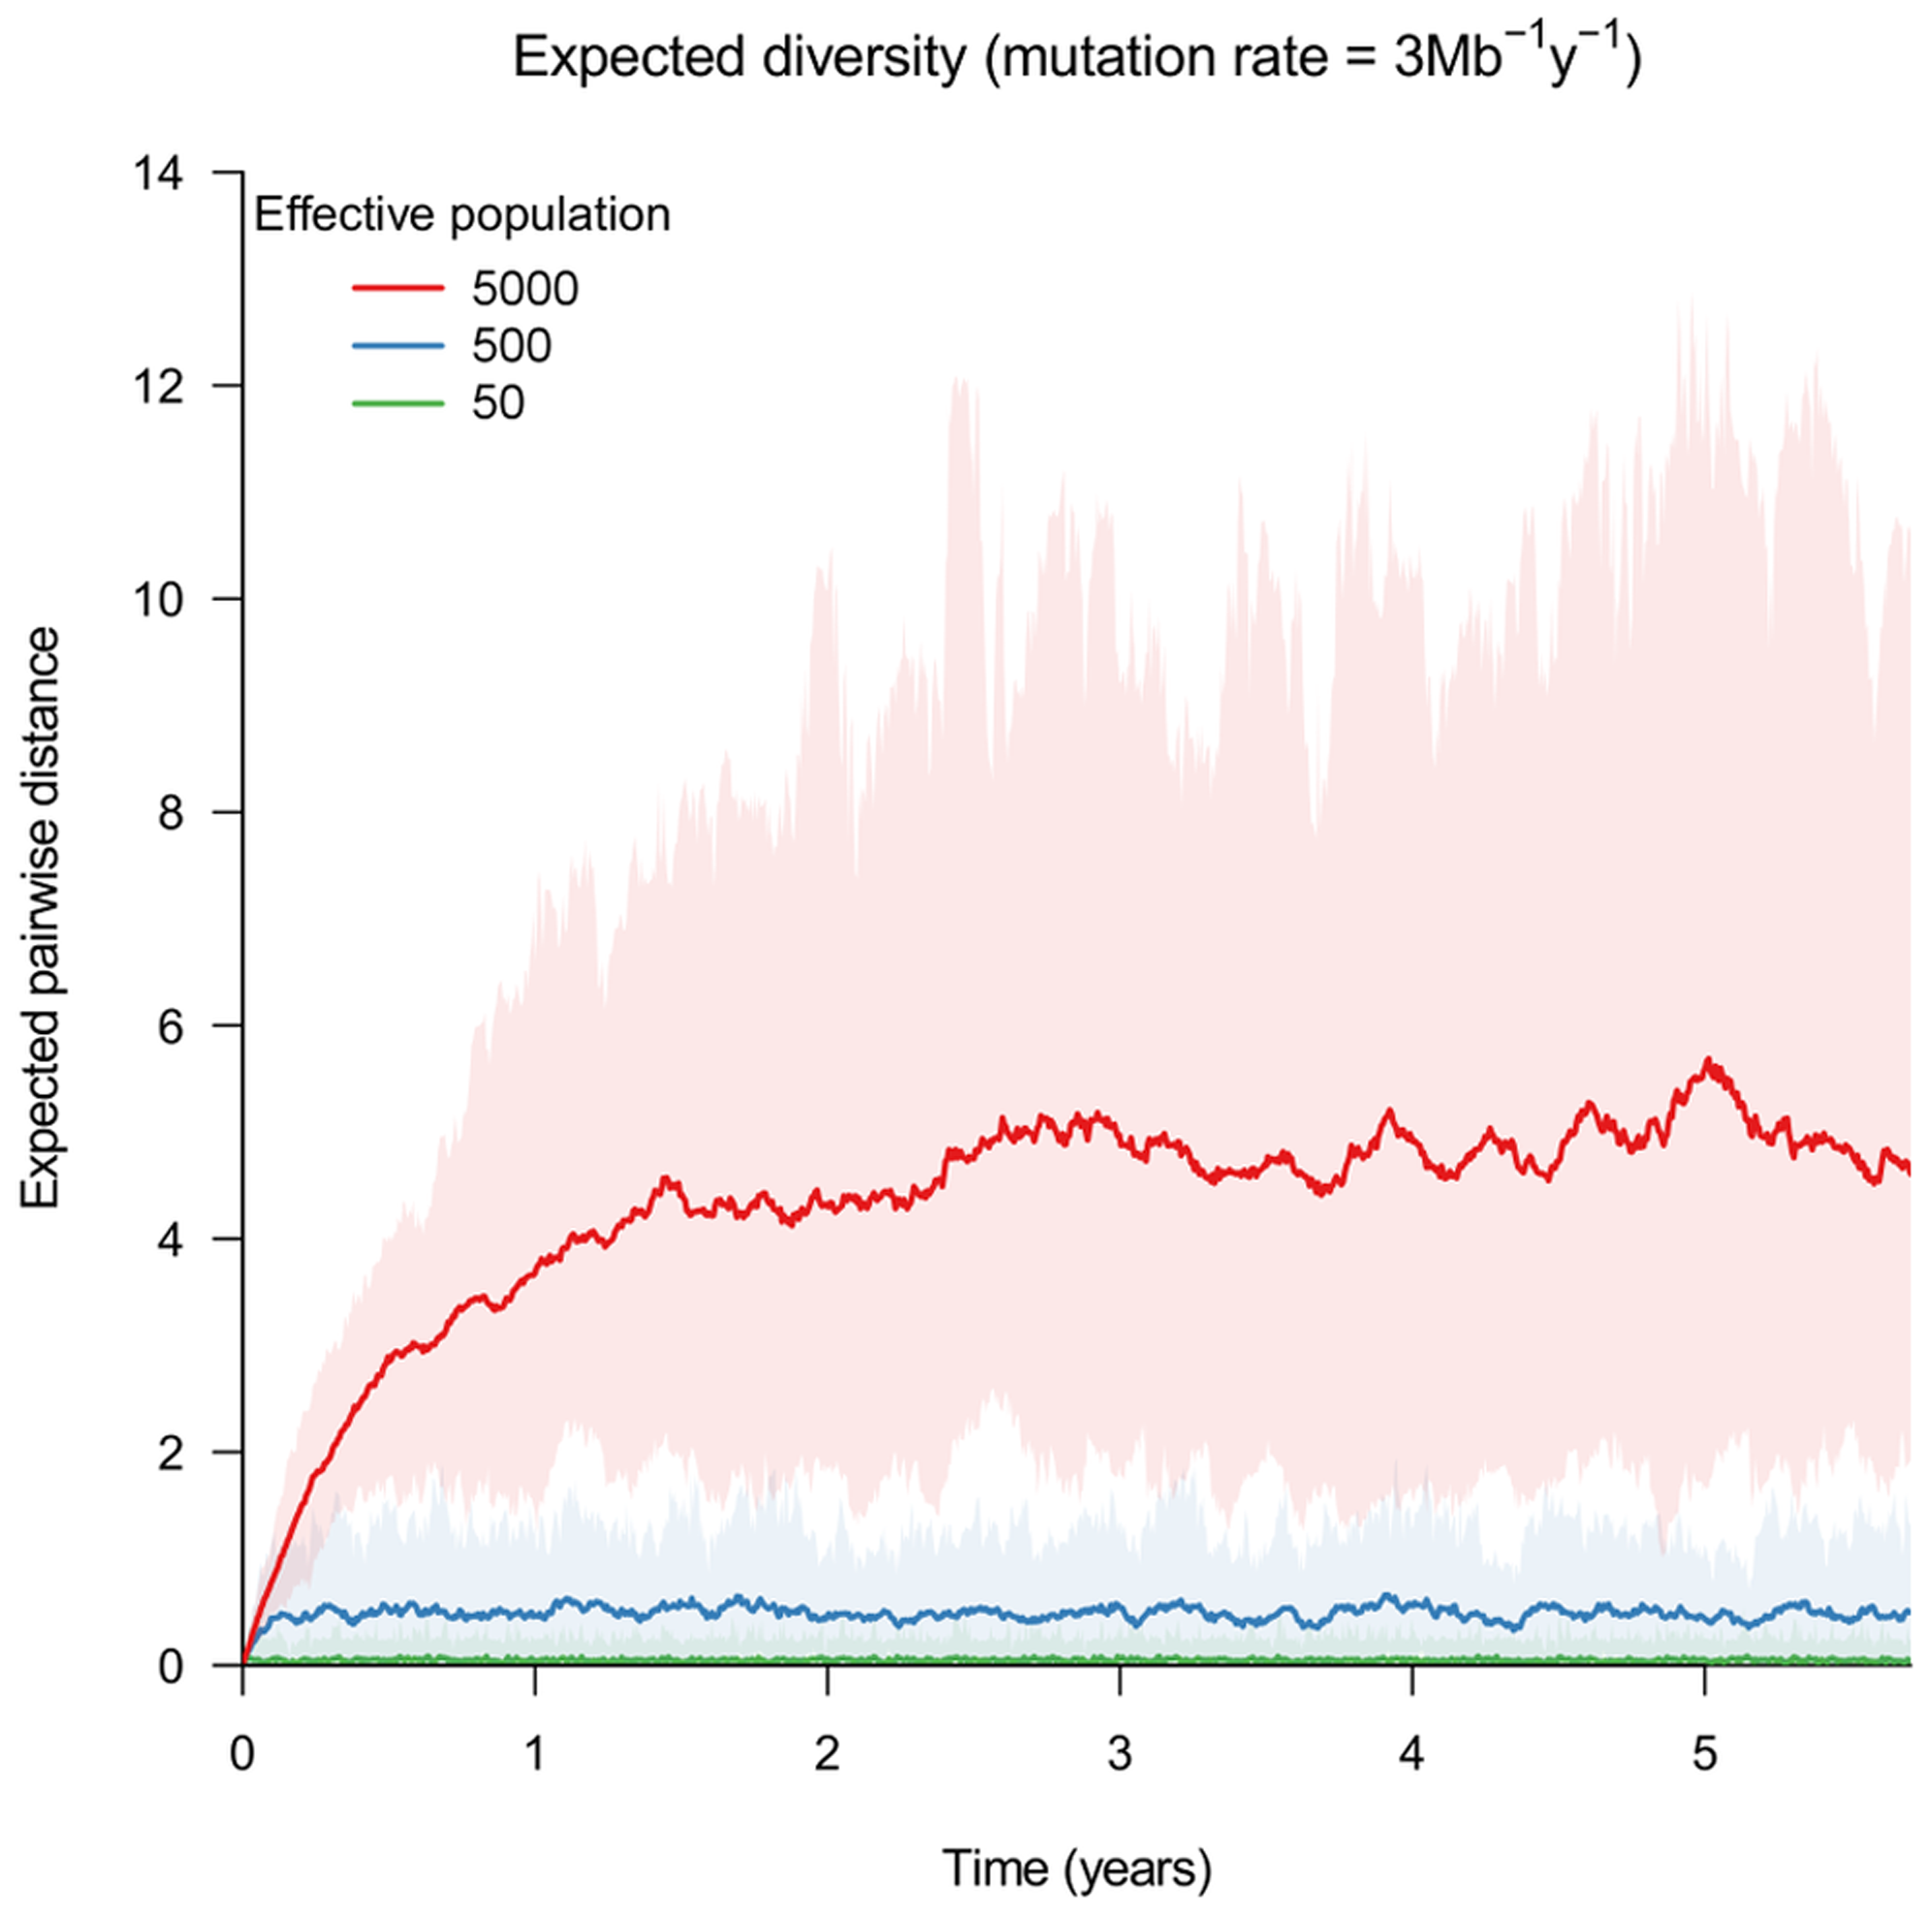
\includegraphics[width=\textwidth]{f1}
        \end{column}
    \end{columns}
\end{frame}

\begin{frame}{Bottlenecks in transmission chains reduce diversity}
    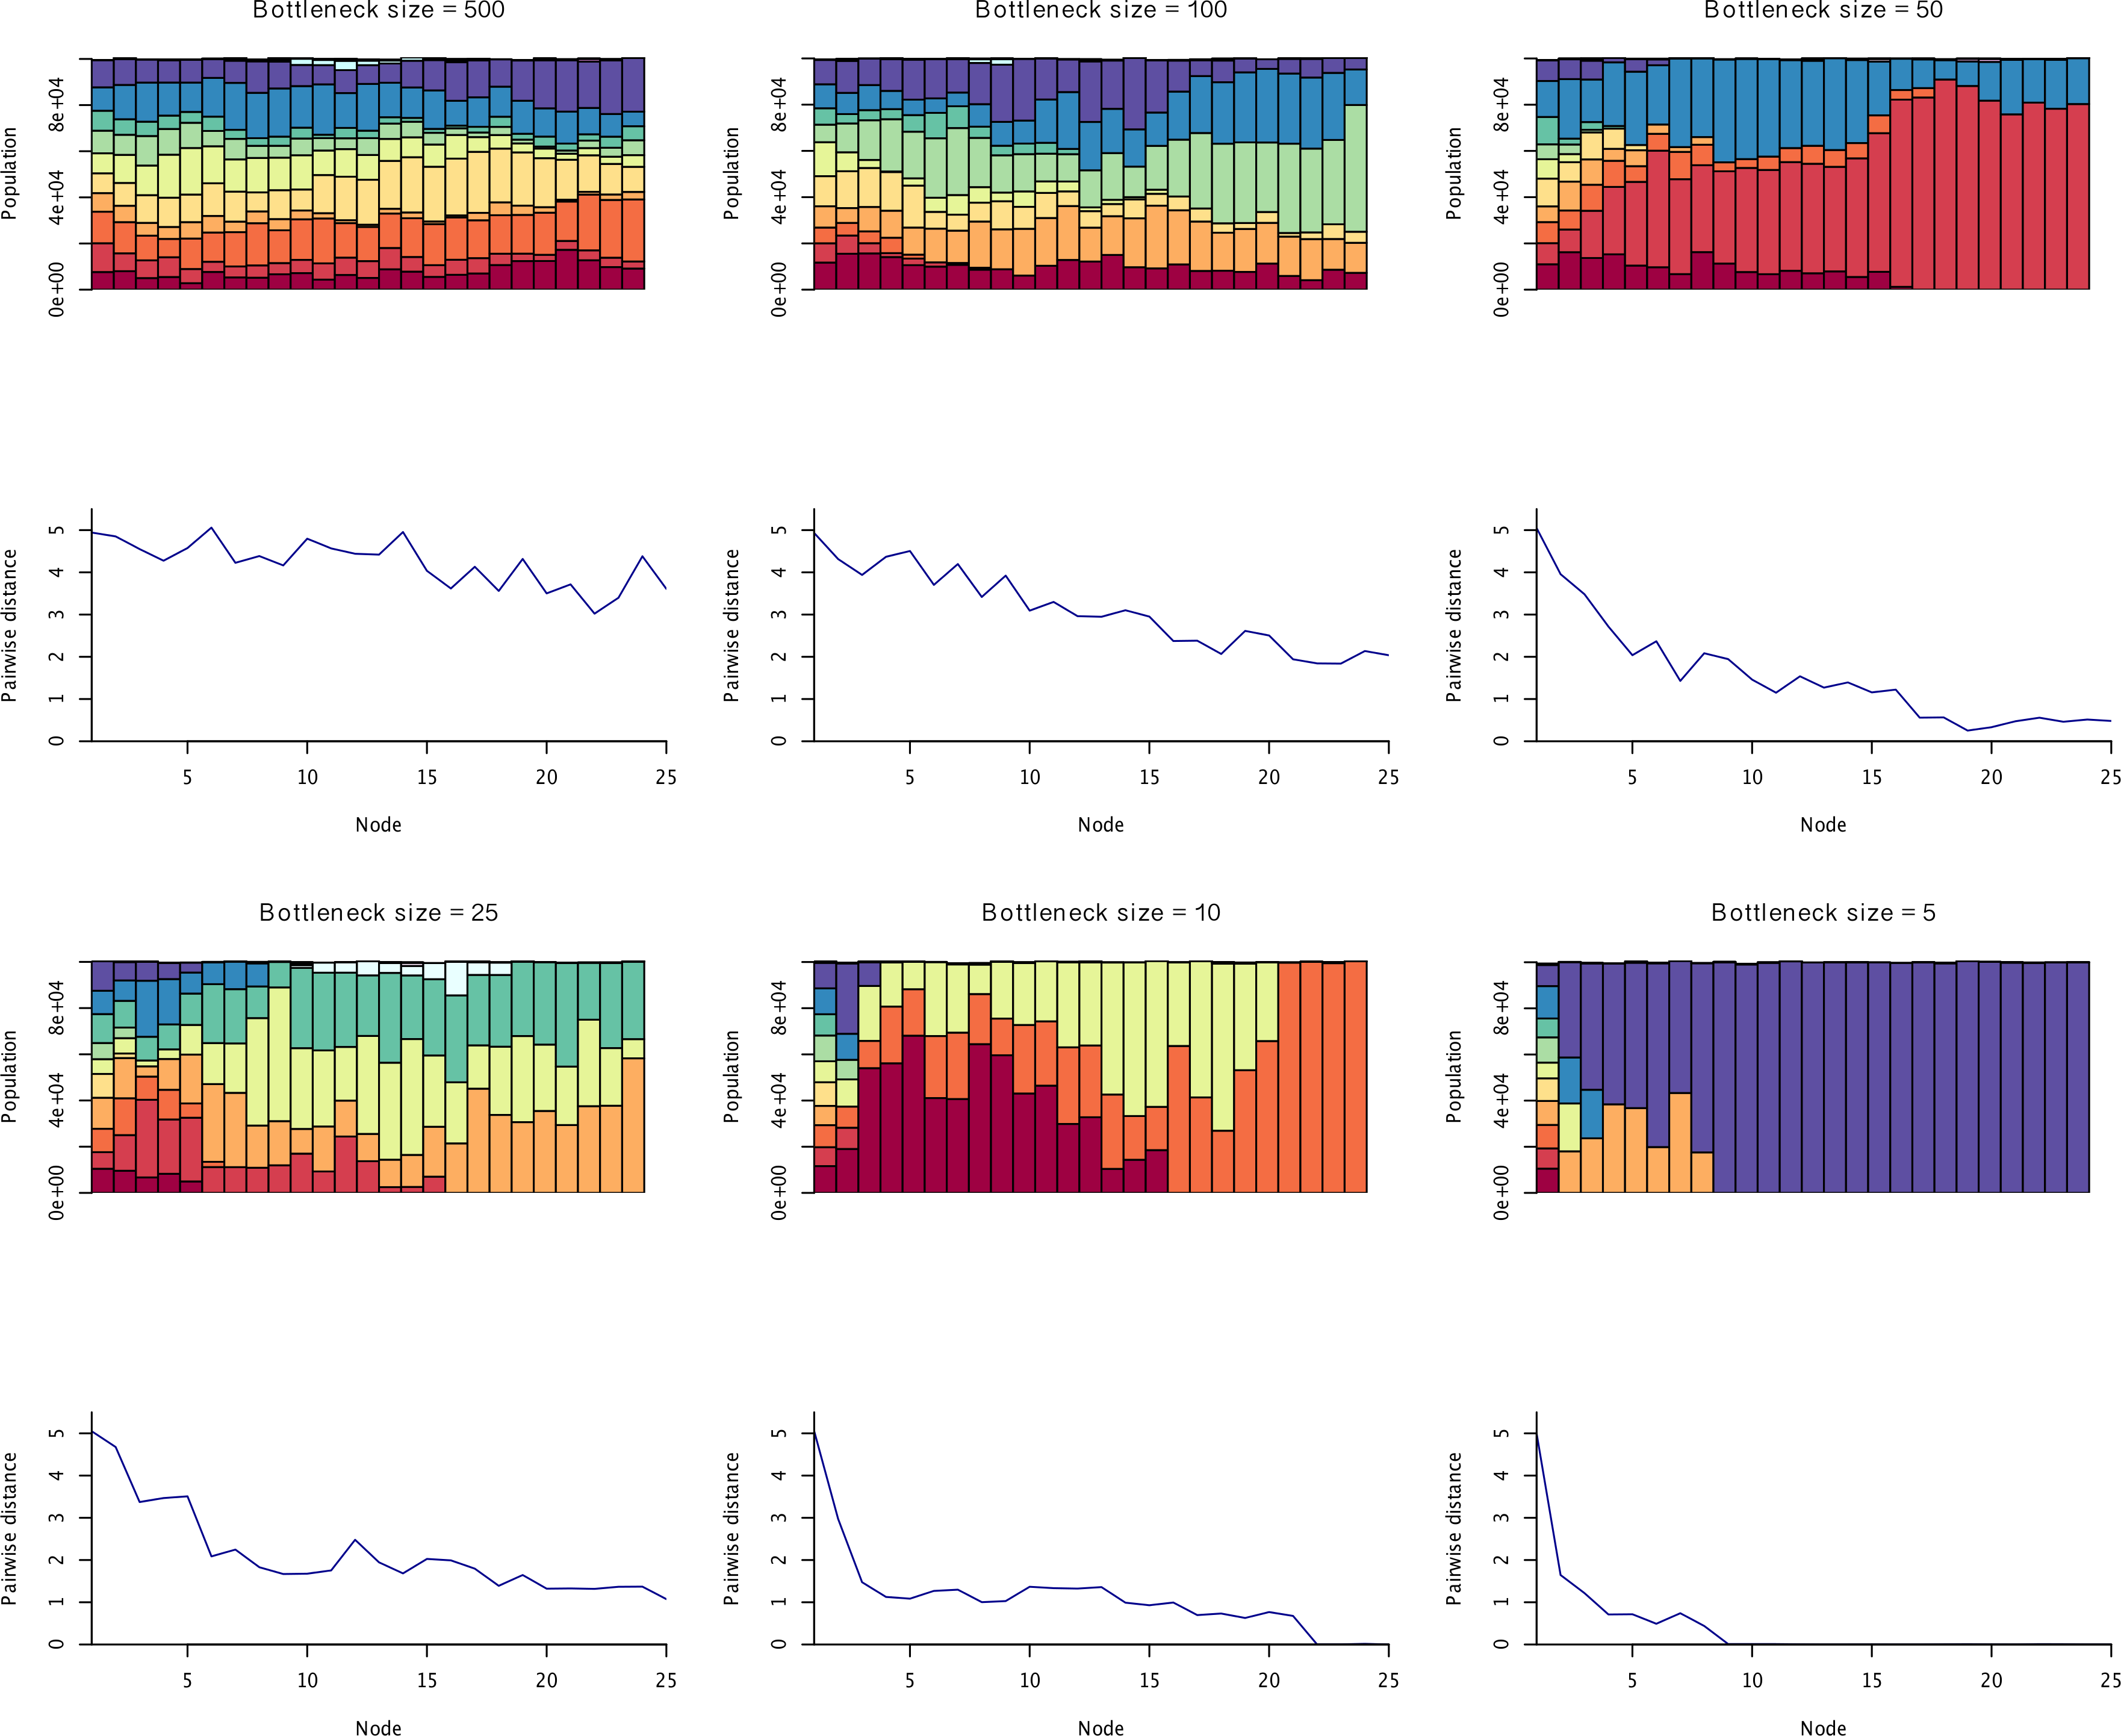
\includegraphics[trim=0 2in 0 0, clip=true, width=\textwidth]{fs3}
\end{frame}

\begin{frame}{High mutation rate mitigates loss of diversity}
    \vspace{-0.5cm}
    \begin{center}
        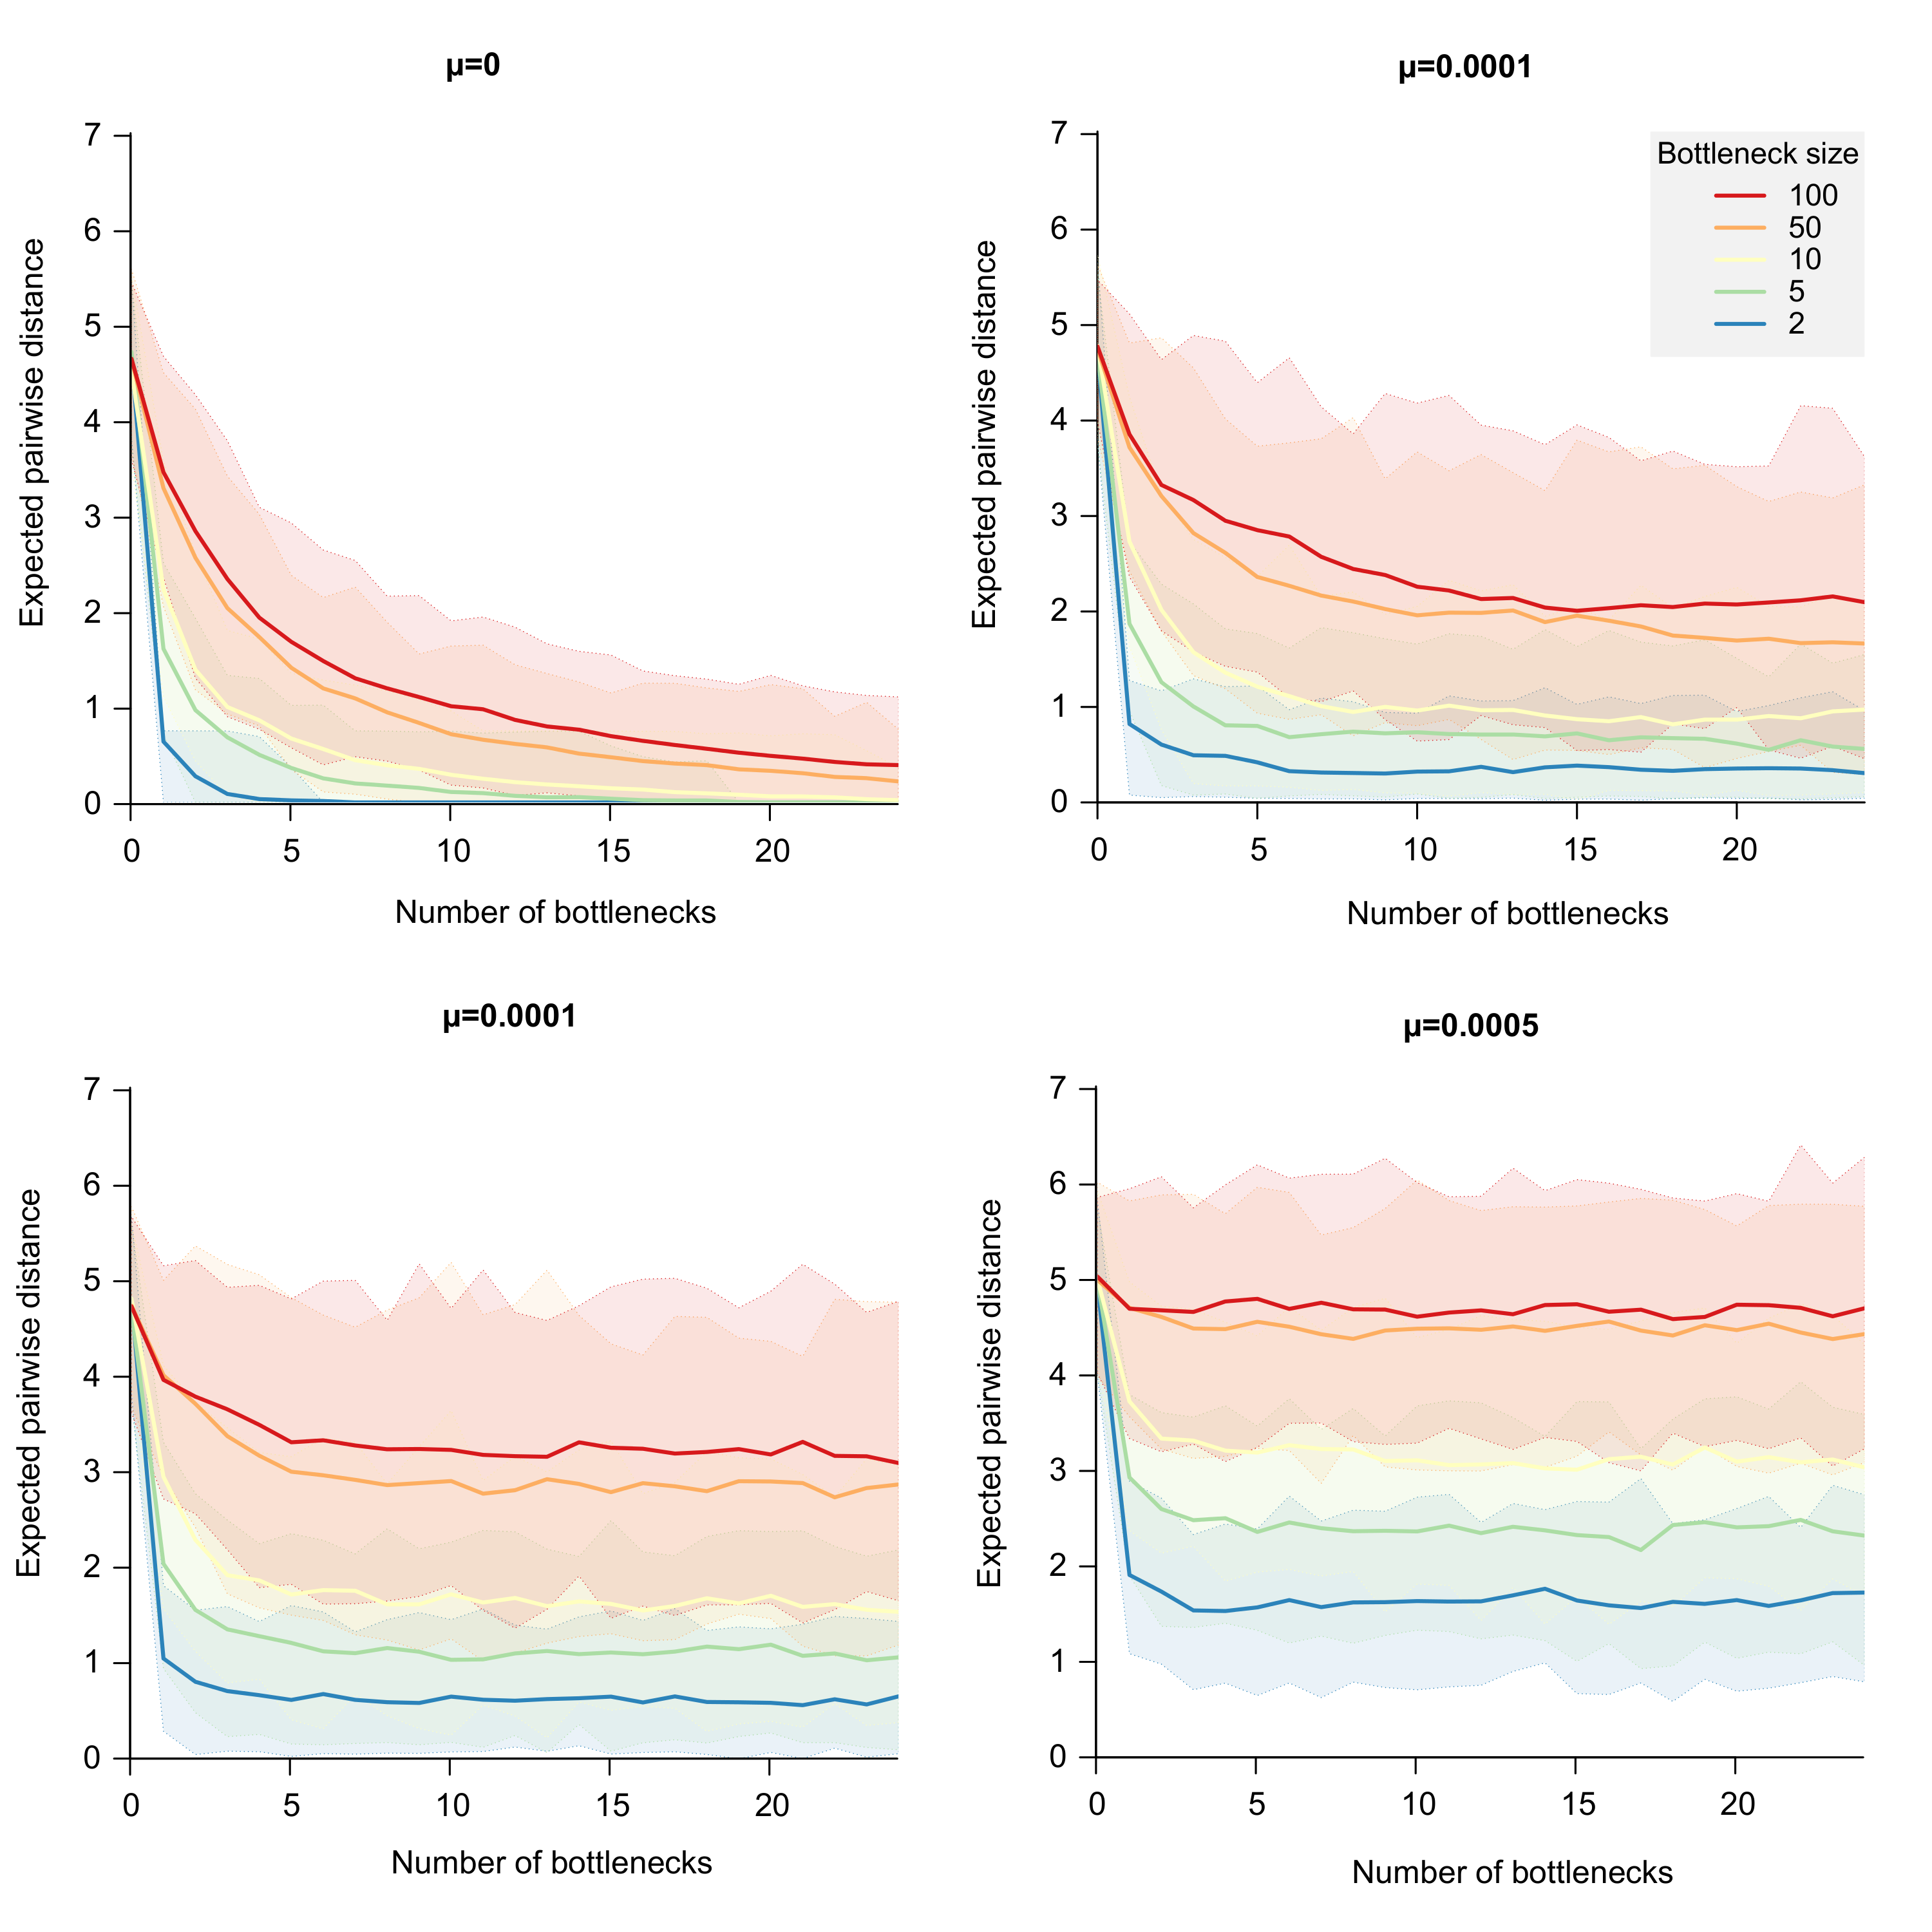
\includegraphics[scale=0.3]{fs4}
    \end{center}
\end{frame}

\begin{frame}{Simulated transmission chains}
    \begin{itemize}
        \setlength{\itemsep}{10pt}
        \item Transmissions occur every 1000 bacterial generations.
        \item Upon infection, an inoculum of size $N_B$ is transferred from the
            source to the target.
        \item Order of infection is known.
        \item All infected individuals are observed and periodically sampled.
        \item Reconstructed transmission links: probability of transmission is
            inversely proportional to mean pairwise genetic distance.
    \end{itemize}
\end{frame}

\begin{frame}{More sampling = better reconstruction}
    \begin{center}
        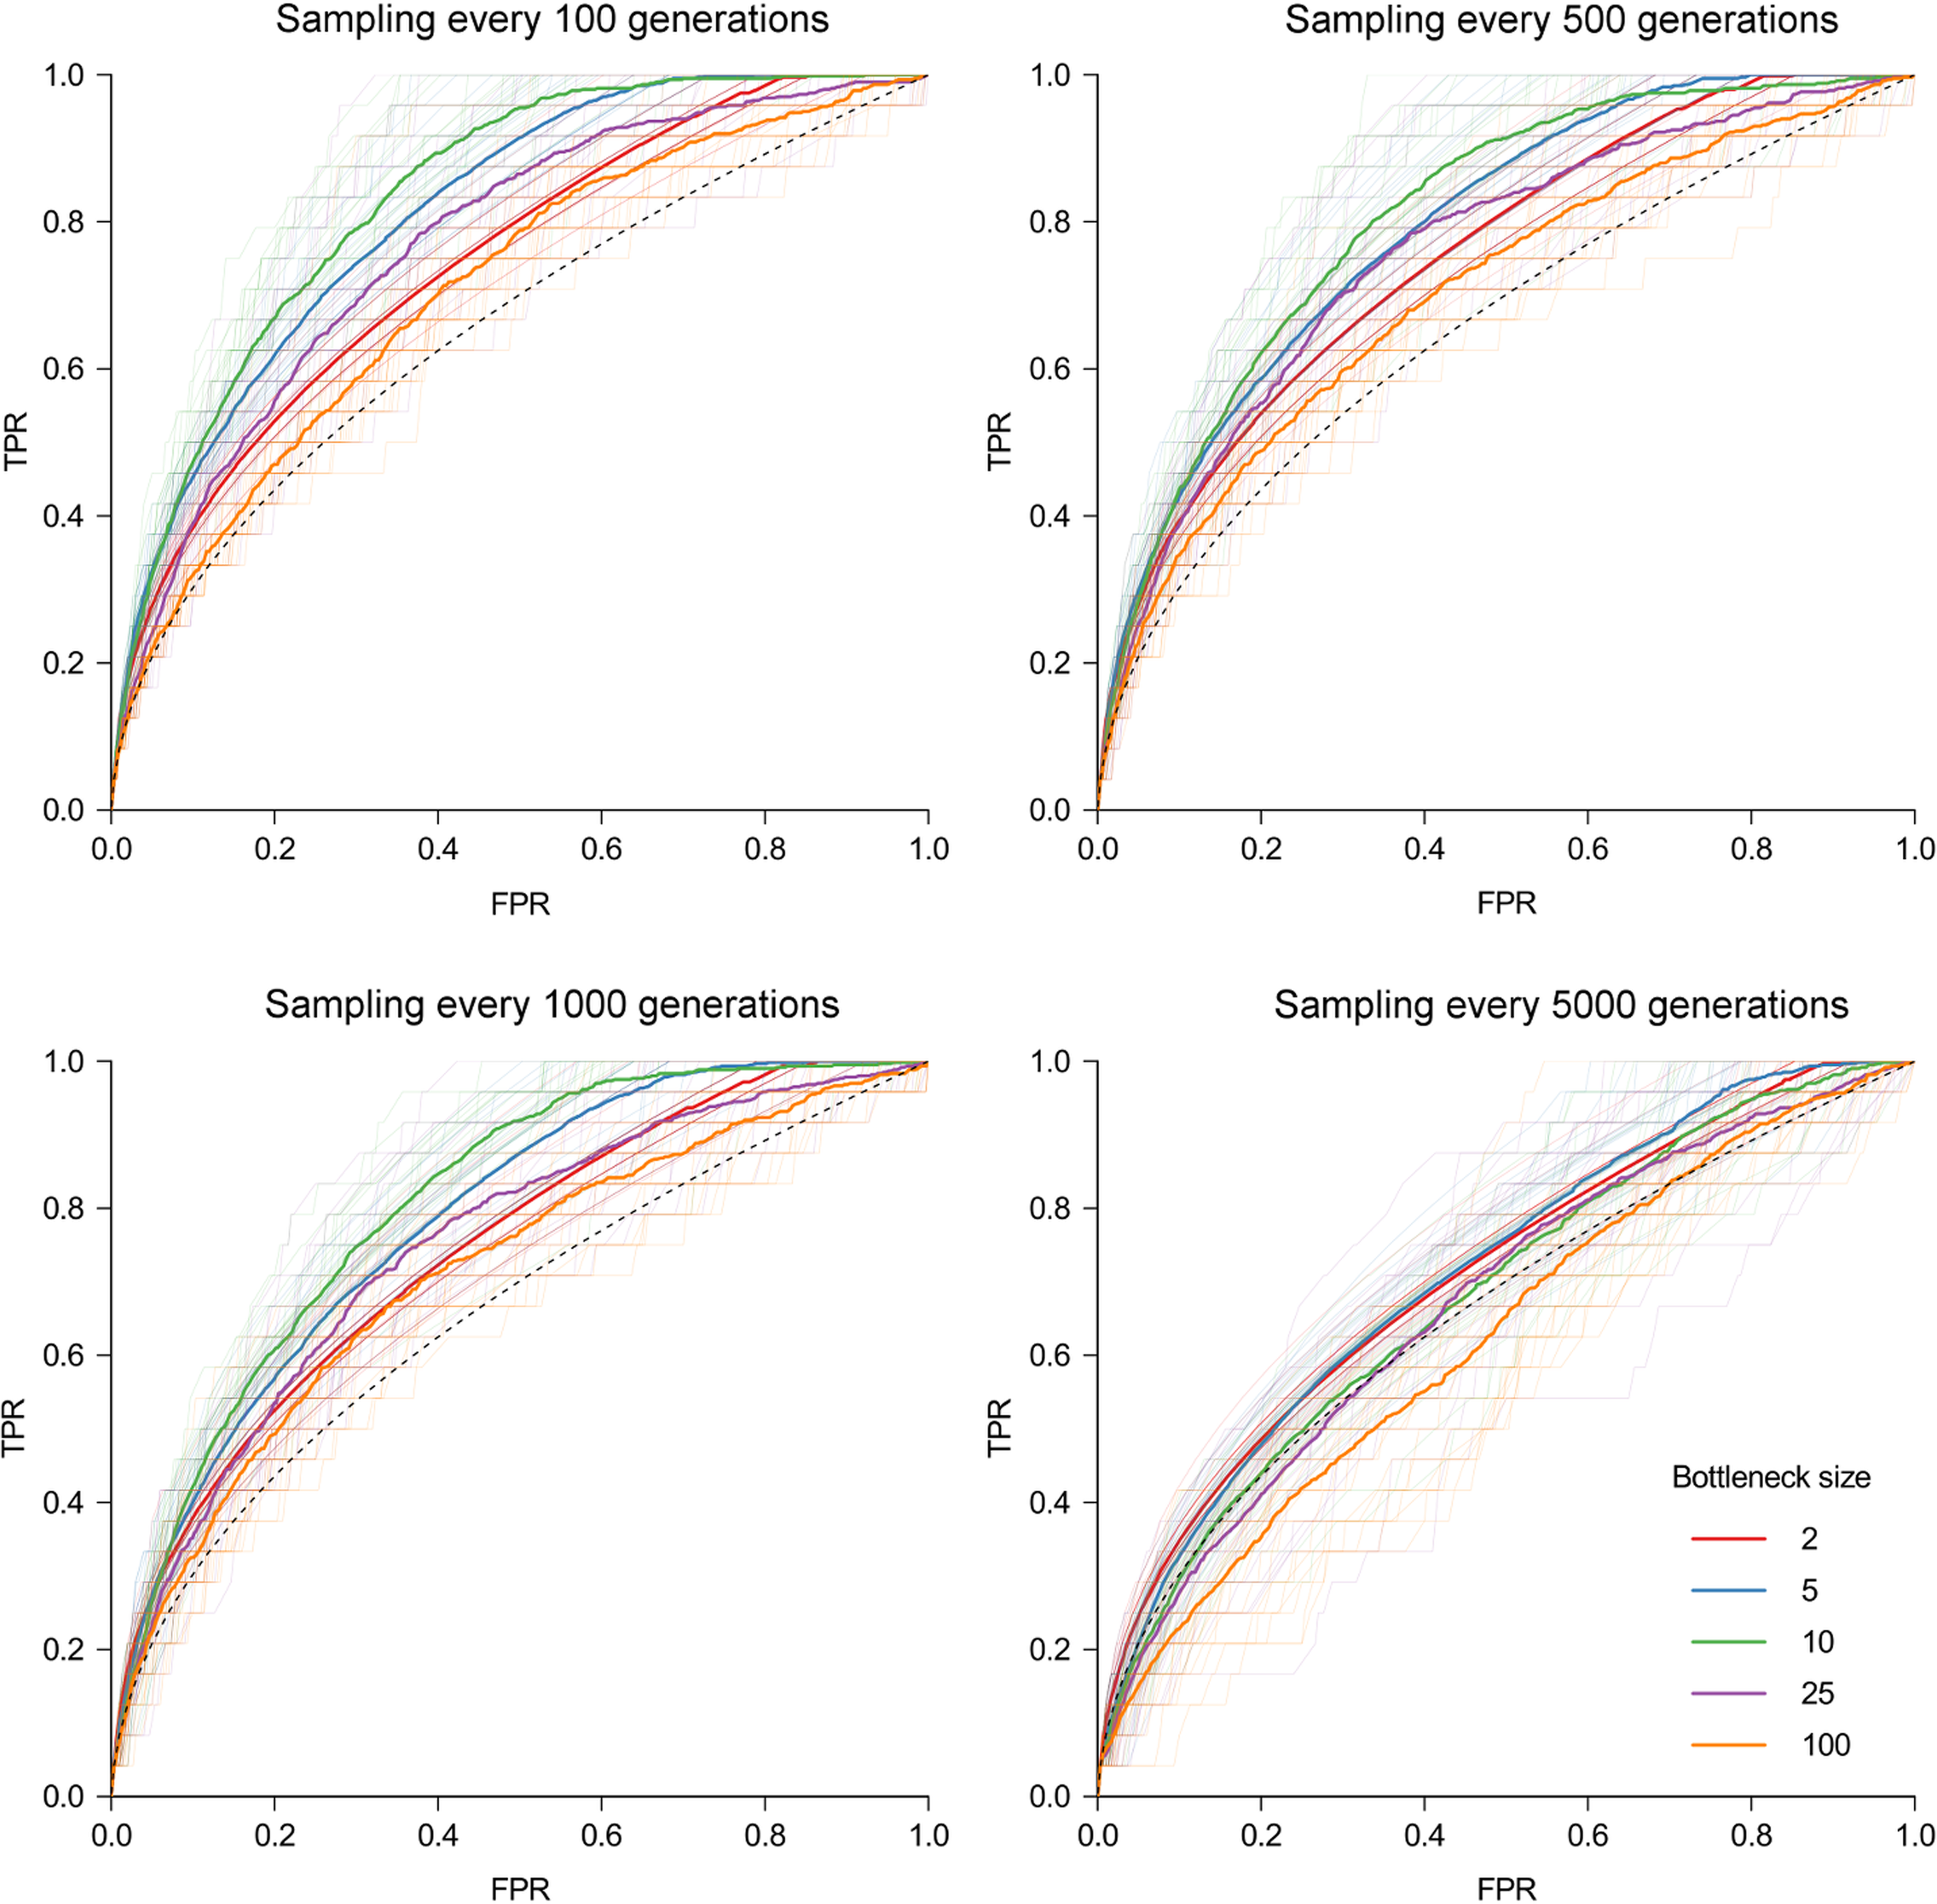
\includegraphics[scale=1.5]{f3}
    \end{center}
\end{frame}

\begin{frame}{Simulated epidemics}
    \begin{columns}
        \begin{column}{0.5\textwidth}
            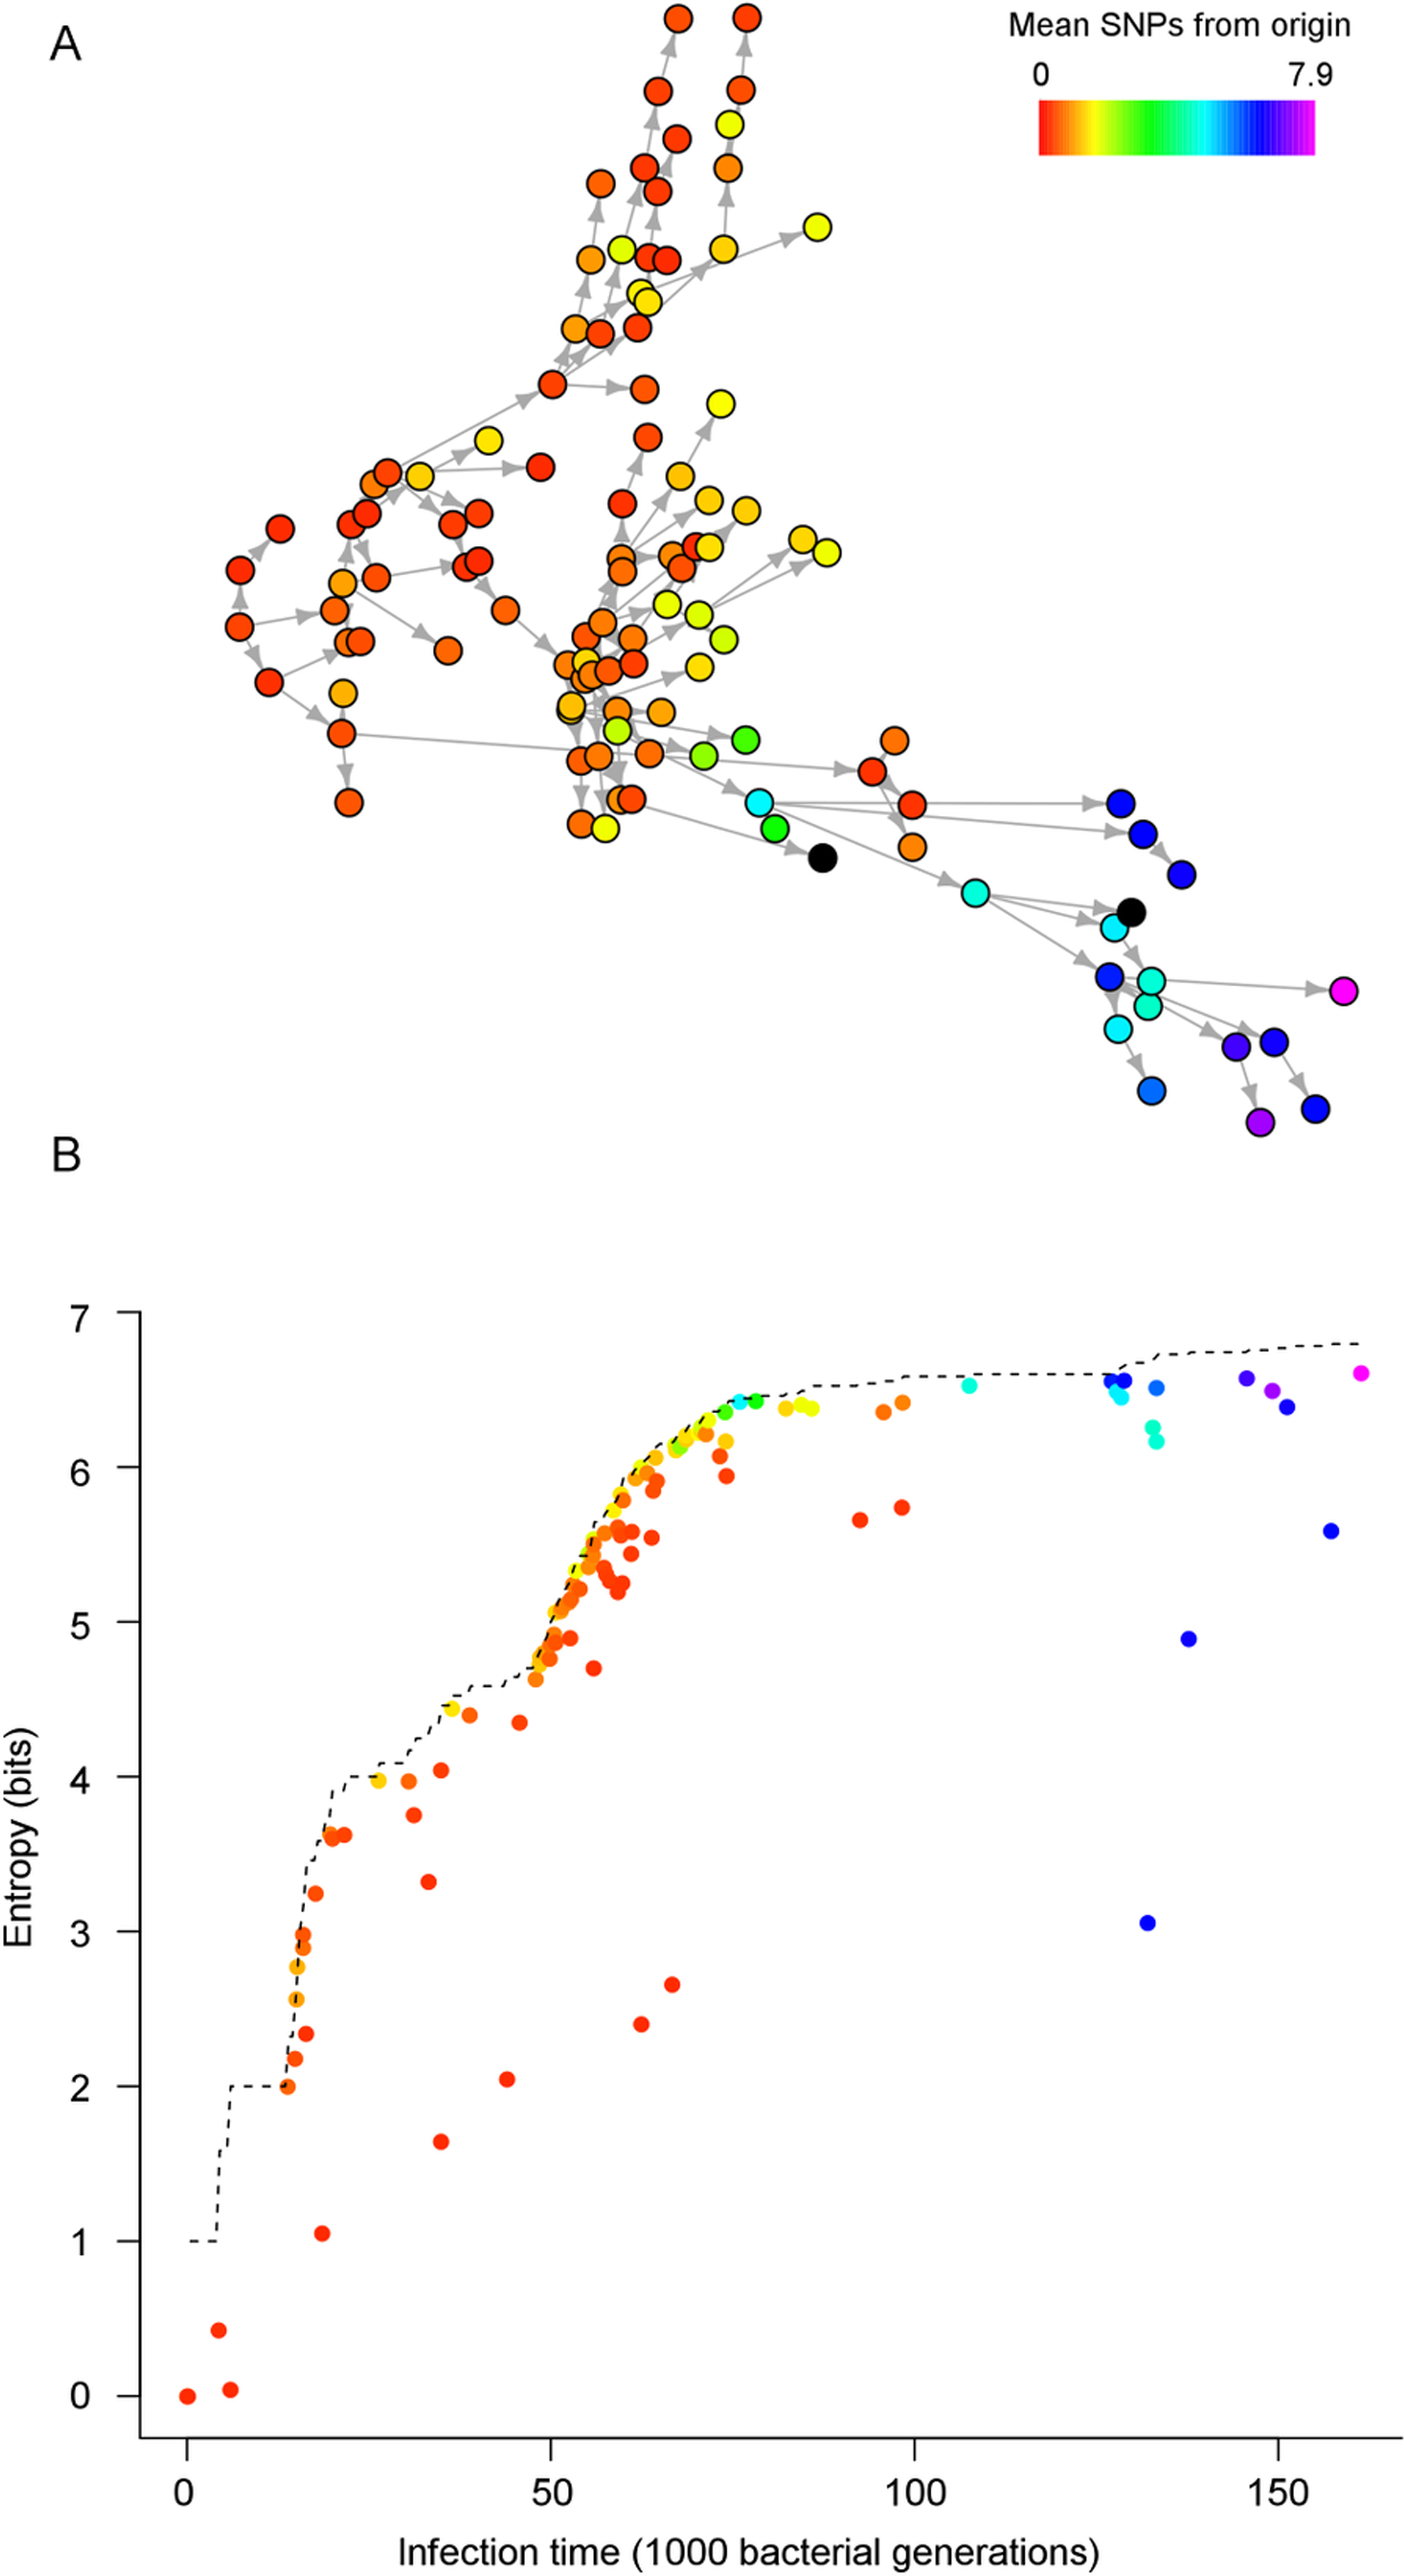
\includegraphics[width=\textwidth, trim=0 1.3in 0 0, clip=true]{f4}
        \end{column}
        \begin{column}{0.5\textwidth}
            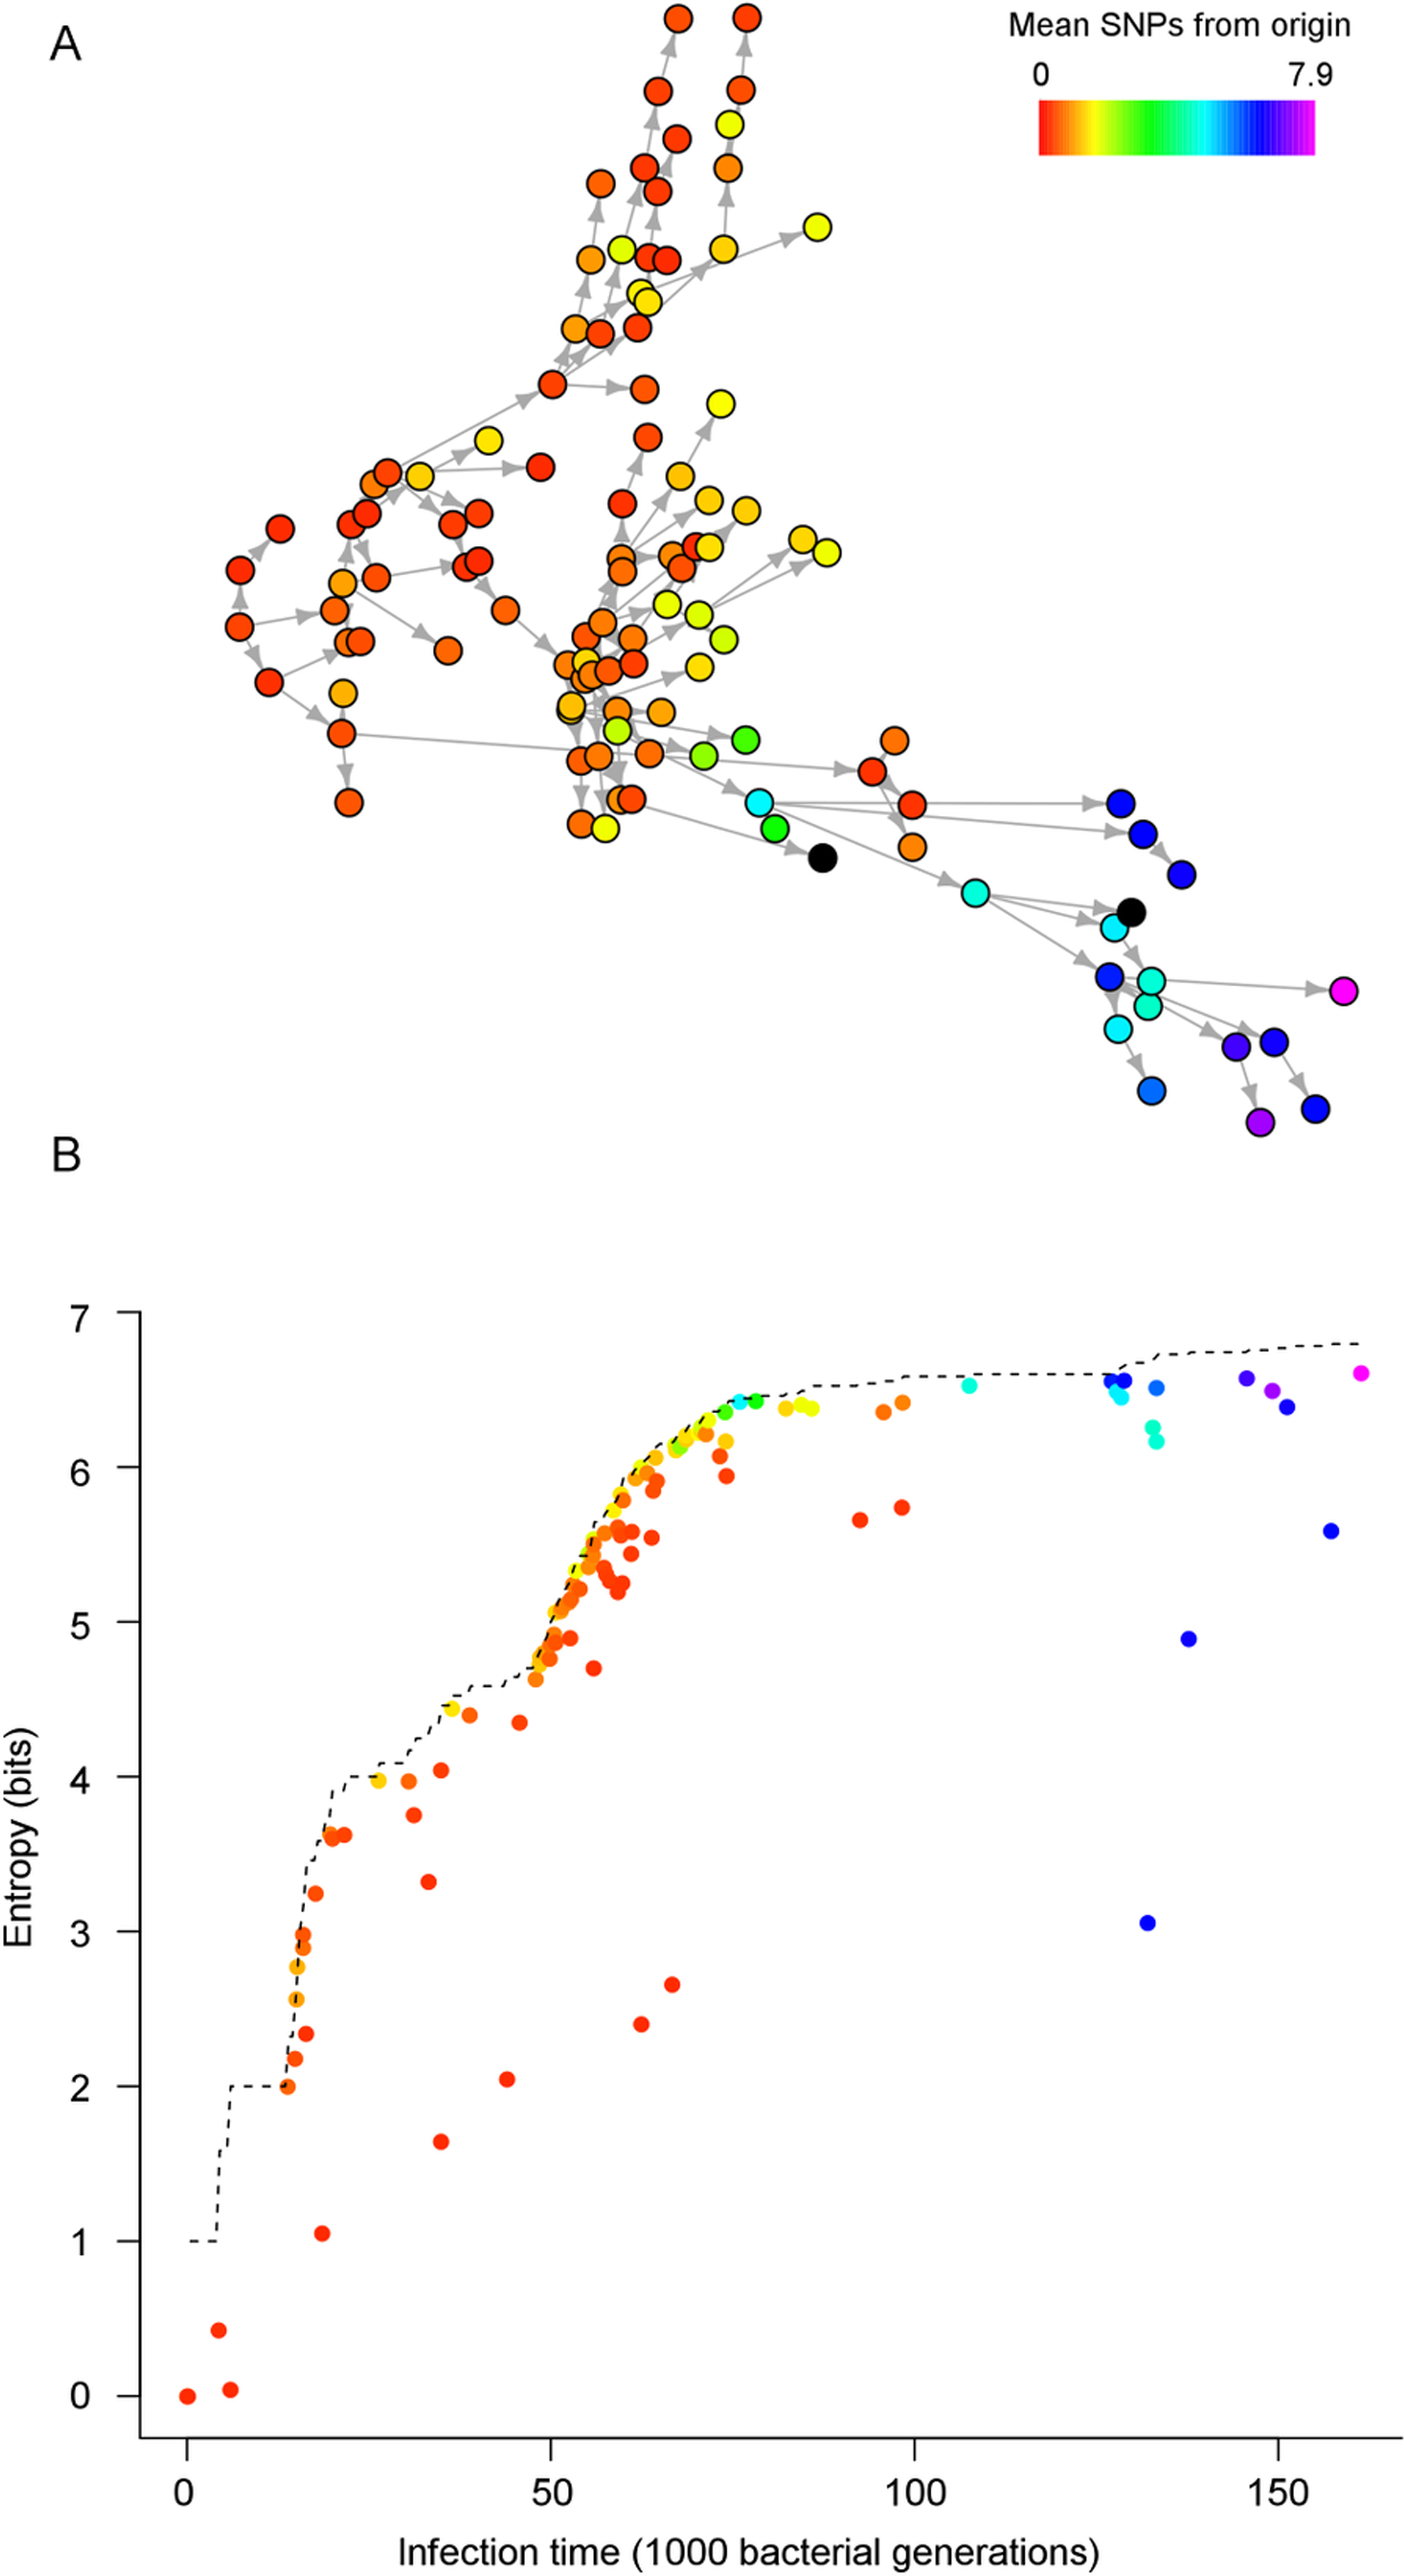
\includegraphics[width=\textwidth, trim=0 0 0 1.1in, clip=true]{f4}
        \end{column}
    \end{columns}

    \begin{center}
        Diversity increases with distance from epidemic source (obviously?).
    \end{center}
\end{frame}

\begin{frame}{Importance factors}
    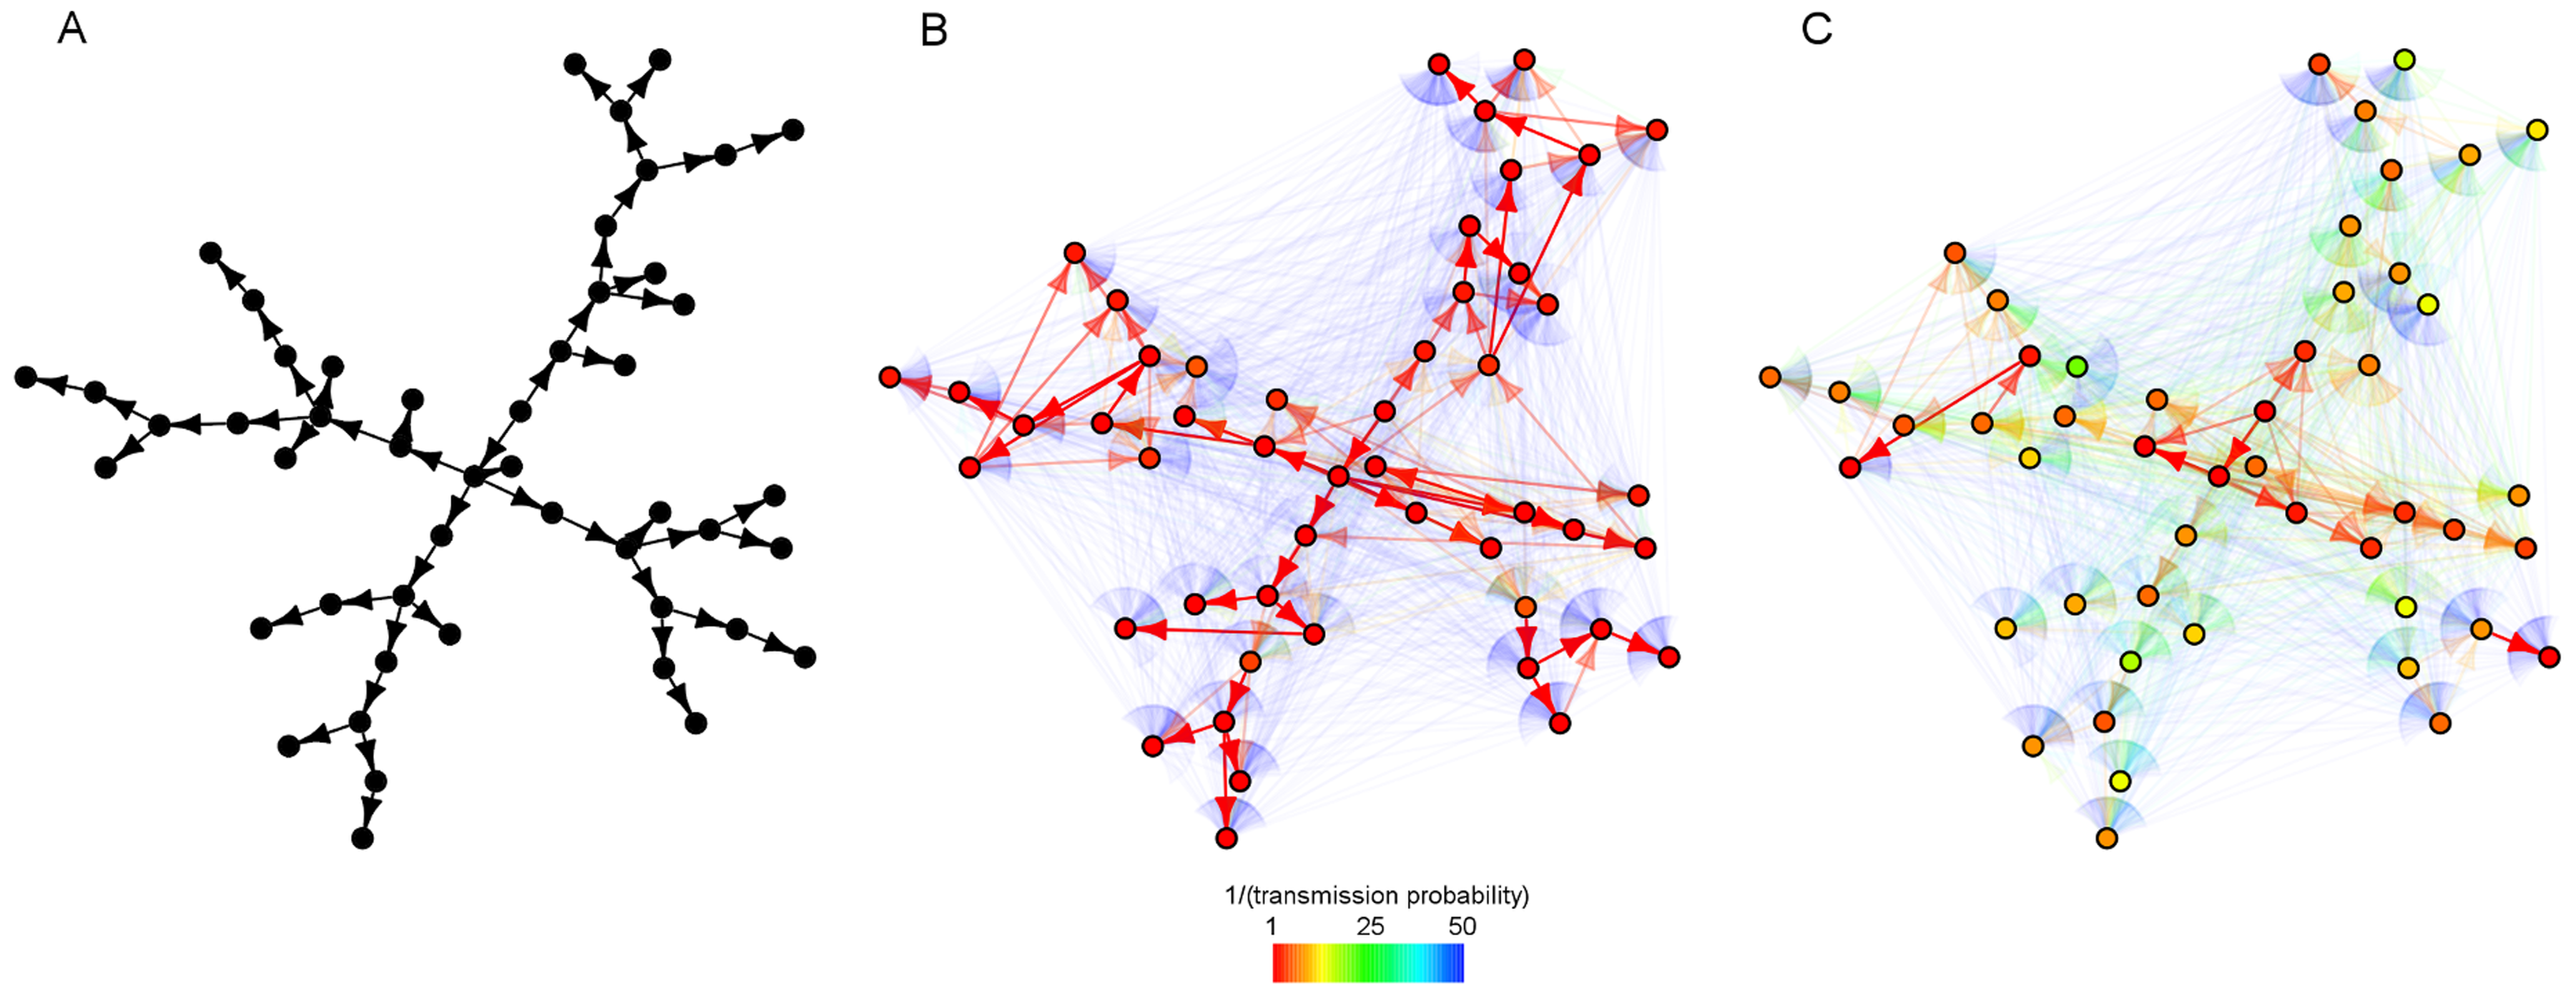
\includegraphics[width=\textwidth]{f5}

    \begin{center}
        Assigning greater importance to genetic similarity increases precision
        at the expense of accuracy.
    \end{center}
\end{frame}

\end{document}
